\documentclass{article}
\usepackage{setspace,tikz,wrapfig}
\usepackage[text={6.5in,8.5in},centering]{geometry}
\geometry{verbose,a4paper,tmargin=2.4cm,bmargin=2.4cm,lmargin=2.4cm,rmargin=2.4cm}
\usepackage{graphicx,amsmath,cases,multirow,appendix,graphicx,xcolor}

\setlength\parindent{0pt}

\newcommand{\note}[1]{\colorbox{gray!30}{#1}}
\newcommand{\ind}{\-\hspace{1cm}}
\newcommand*\circled[1]{\tikz[baseline=(char.base)]{
            \node[shape=circle,draw,inner sep=2pt] (char) {#1};}}
\newenvironment{rcases}
  {\left.\begin{aligned}}
  {\end{aligned}\right\rbrace} 
  
  
\renewcommand\floatpagefraction{.9}
\renewcommand\topfraction{.9}
\renewcommand\bottomfraction{.9}           


\begin{document}

\noindent\makebox[\textwidth][c]{\Large\bfseries Lecture 14 -- Ruth-Hurwitz Criteria}

\textbf{Concepts:}\\
\ind - Determinant, Traces \& Routh-Hurwitz criteria\\
\ind - Paper discussion

\rule[0.5ex]{\linewidth}{1pt}

\textbf{Back to Biology:  Classifying steady states}\\
For 2x2 system:
\begin{equation*}
	\lambda^2 - \underbrace{(A_{11}+A_{22})}_{\text{Trace}}\lambda + \underbrace{A_{11}A_{22} - A_{12}A_{21}}_{\text{Determinant}}
\end{equation*}

\textbf{Routh-Hurwitz stabiliy criteria}\\
\ind \ind Provide \emph{biological insight} (far more challenging using just $\lambda$'s)\\
\ind \ind Unfortunately, the simplicity of the following applies only to 2 x 2 systems.\\

\ind Tr$(\mathbf{A})<0 \quad \Rightarrow \quad A_{11}+A_{22}<0$ is necessary for stability\\
\ind \ind $\Rightarrow$ \emph{At least some species must be strongly self-limiting for stability} $\Leftarrow$ \\

\ind Det$(\mathbf{A})>0  \quad \Rightarrow \quad A_{11} A_{22} - A_{12} A_{21} > 0$ is necessary for stability\\
\ind \ind $\Rightarrow$ \emph{Overall self-limitation must be stronger then interspecific effects for stability} $\Leftarrow$\\
\ind \ind $\Rightarrow$ \emph{Intra $>$ inter-specific effects} $\Leftarrow$ \\

Each condition by itself is \emph{necessary, but not sufficient}.
\begin{equation*}
	\lambda = \tfrac{1}{2}\text{Tr}(\textbf{A}) \pm \tfrac{1}{2}\sqrt{(-\text{Tr}(\textbf{A}))^2 - 4\cdot\text{Det}(\textbf{A})}
\end{equation*}

\ind Whichever parts of $\sqrt{\phantom{x}}$ is bigger determines with or without oscillations.\\
\ind Bifurcation occurs at $(-\text{Tr}(\textbf{A}))^2 = 4\cdot \text{Det}(\textbf{A})$.\\
\begin{center}
 	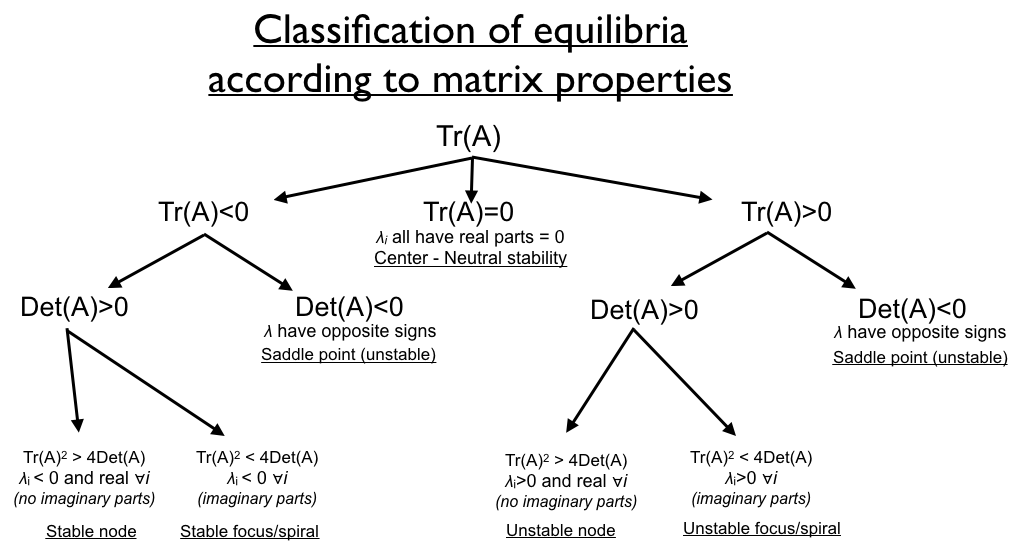
\includegraphics[width=16cm]{figs/Classify}
\end{center}
 
\rule[0.5ex]{\linewidth}{1pt}
\pagebreak

\textbf{Rosenzweig-MacArthur paradox of enrichment model - revisited}
\begin{equation*}
	\frac{dR}{dt}=rR\left( 1-\frac{R}{K}\right) - \frac{aRC}{1+ahR} \qquad \qquad
	\frac{dC}{dt}=\frac{eaRC}{1+ahR} - dC
\end{equation*}

Prey isocline:
\begin{equation*}
	\frac{dR}{dt}=0 \quad \Rightarrow \quad C^*= \frac{r(K-R)(1-ahR)}{aK}
\end{equation*}

Predator isocline:
\begin{equation*}
	\frac{dC}{dt}=0 \quad \Rightarrow \quad R^* = \frac{d}{a(e-dh)}
\end{equation*}
 \begin{center}
 	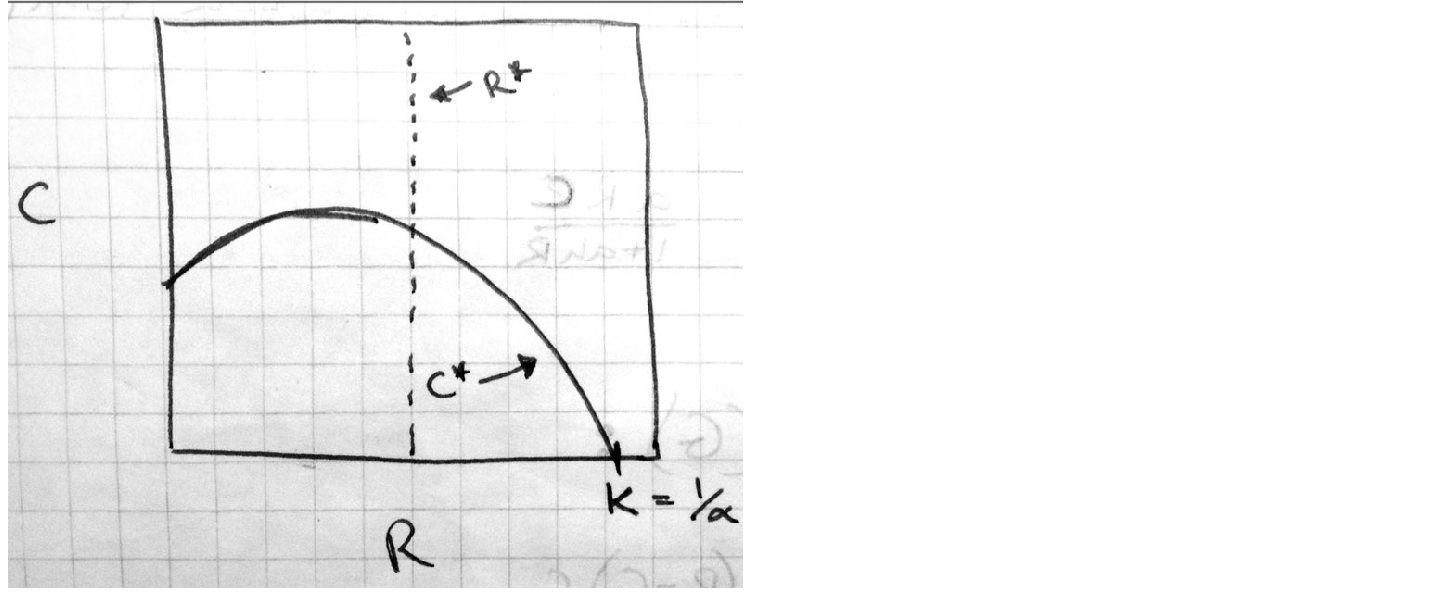
\includegraphics[width=6cm]{figs/MRiso.pdf}
 \end{center}

When $ R* > K \Rightarrow$ predator extinct\\
Increasing $K$ shifts $C^*$ to right\\
\ind When $R^*> \max C^* \Rightarrow$ stable fixed point\\
\ind When $R^*< \max C^* \Rightarrow$ stable limit cycle\\
\ind \ind = \emph{Hopf bifurcation}
\begin{center}
 	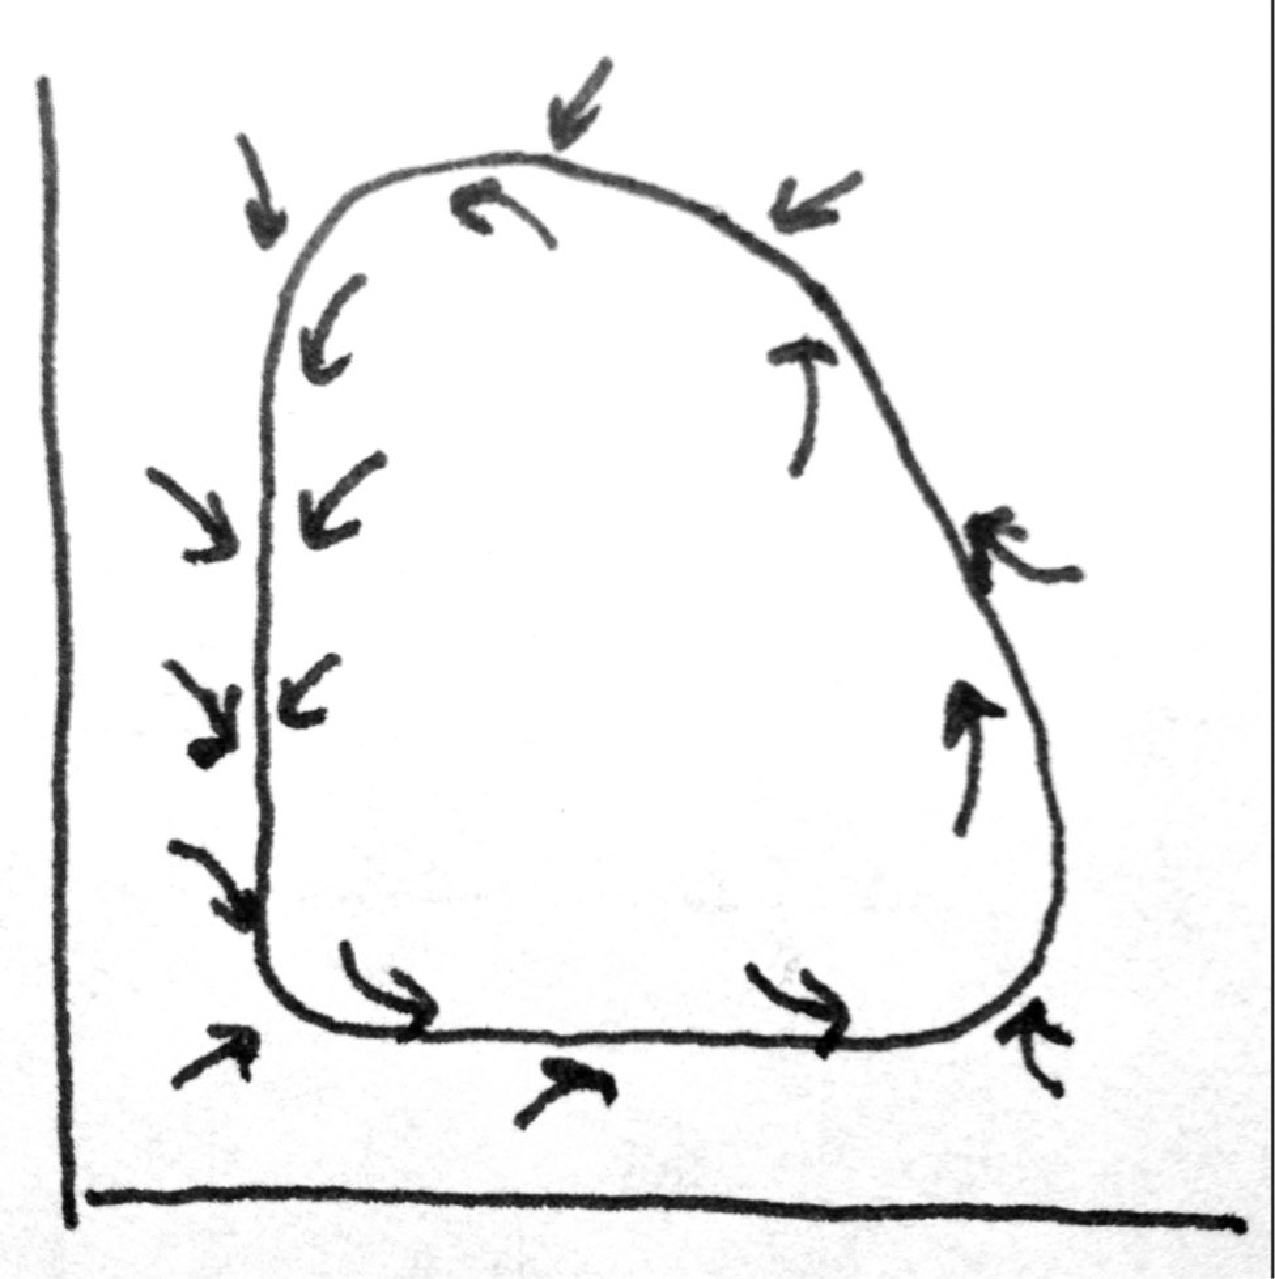
\includegraphics[width=5cm]{figs/LimitCycle.pdf}
\end{center}
\textbf{Key control parameters:}\\
As $K$ increases, oscillation amplitude increases $\Rightarrow$ Risk of extinction\\
$h$ influences position of $R^*$ and how hump-shaped $C^*$ is.\\

Note: If $h=0 \Rightarrow C^* = \frac{r(K-R)}{aK}$, just like LV but with logistic prey:
\begin{center}
 	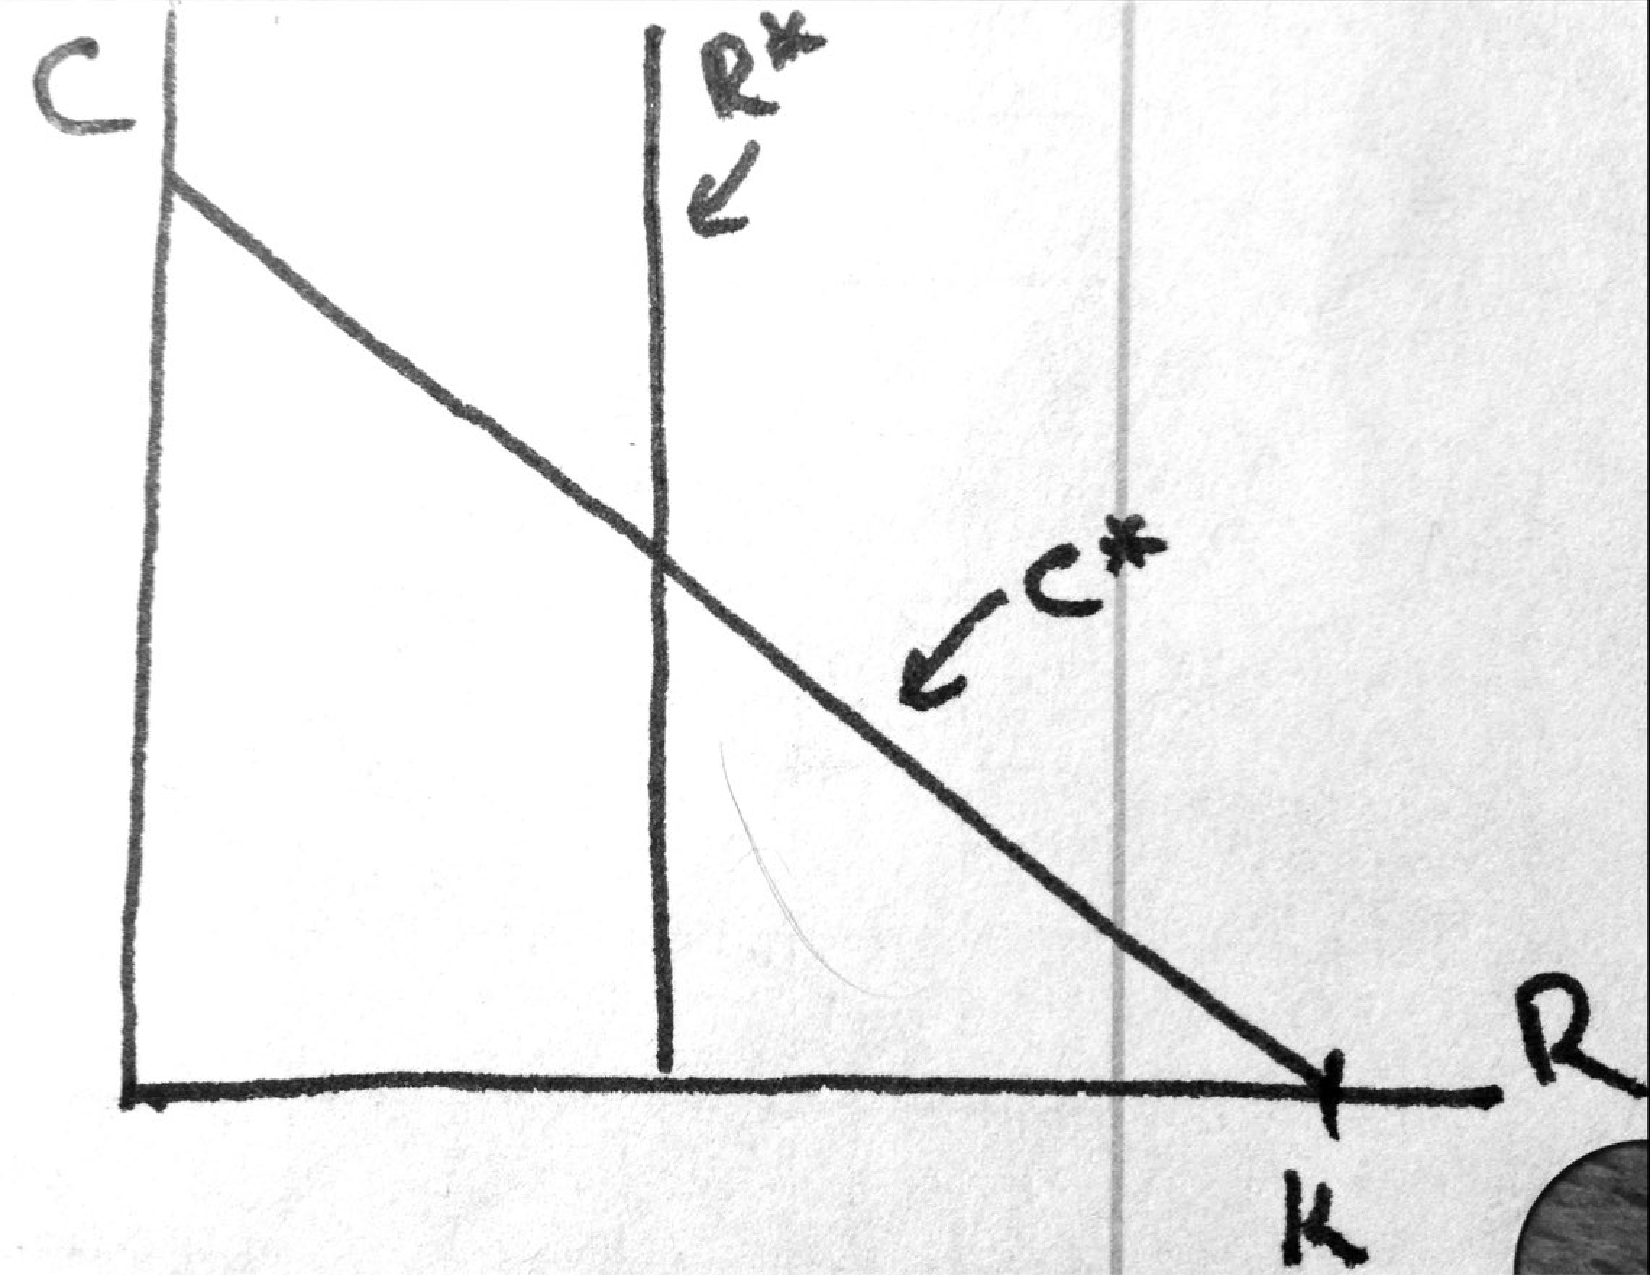
\includegraphics[width=6cm]{figs/LVlog.pdf}
\end{center}
Other parameters are less interesting for today.

\rule[0.5ex]{\linewidth}{1pt}

\pagebreak

\textbf{Formal stability analysis}\\
\textbf{Step 1:} Solve for steady state equilibria: \note{\emph{Mathematica}}\\
\ind Three solutions:
\begin{equation*}
	(R^*,C^*)=\begin{cases}
	0 & 0\\
	K & 0\\
	\frac{d}{a(e-dh)} & \frac{er(aeK-d-adhK)}{Ka^2(e-dh)^2}
	\end{cases}
\end{equation*}

\textbf{Step 2:} Evaluate Jacobian at steady state(s)\\
\ind Interested only in coexistence, so focus on 3rd
\begin{align*}
	\left.\mathbf{A}\right\vert_{R^*,C^*} 
	&= \begin{bmatrix}r-\frac{2rR^*}{K} - \frac{aC^*}{(1+ahR^*)^2} & \frac{-aR^*}{1+ahR^*}\\
				\frac{eaC^*}{(1+ahR^*)^2} & \frac{eaR^*}{1+ahR}-d \end{bmatrix}\\
	&=\begin{bmatrix} \frac{-dr(e+dh+ahK(dh-e))}{eaK(e-dh)} & \frac{-d}{e}\\
	r\left(e-dh-\frac{d}{aK}\right) & 0 \end{bmatrix}	
	=\begin{bmatrix} A_{11} & A_{12} \\ A_{21}& A_{22}	\end{bmatrix}	
\end{align*}

Note that for this model:\\
\ind $A_{21}$ will always be positive (look at first matrix) - \emph{prey effect on pred}\\
\ind $A_{12}$ will always be negative - \emph{pred effect on prey}\\
\ind $A_{11}$ can be positive or negative depending on $R^*$ and $C^*$\\
\note{Q:} How can $A_{11}>0$?  \note{A:} If $R^*$ and $C^*$ are small, or $K$ is large and $a$ is small.\\
\note{Q:} Why is $A_{22}=0$?  \note{A:} Consumer has no self-limitation (look back at model)\\

\textbf{Step 3:} Assess stability using eigenvalues or Routh-Hurwitz Criteria\\
\ind $\lambda_i <0 \; \forall i \Rightarrow $ Stable fixed point\\
\ind $Tr(\mathbf{A}) < 0 \text{ \& } Det(\mathbf{A})>0 \quad \Rightarrow \quad $ Stable fixed point\\

Graphical analysis:\\
\ind Set $Tr(\mathbf{A})$ \& $Det(\mathbf{A})=0$ and plot as functions of $K$ and $h$:\\
\ind Or plot $Tr(\mathbf{A})$ = $Det(\mathbf{A})$
\begin{center}
 	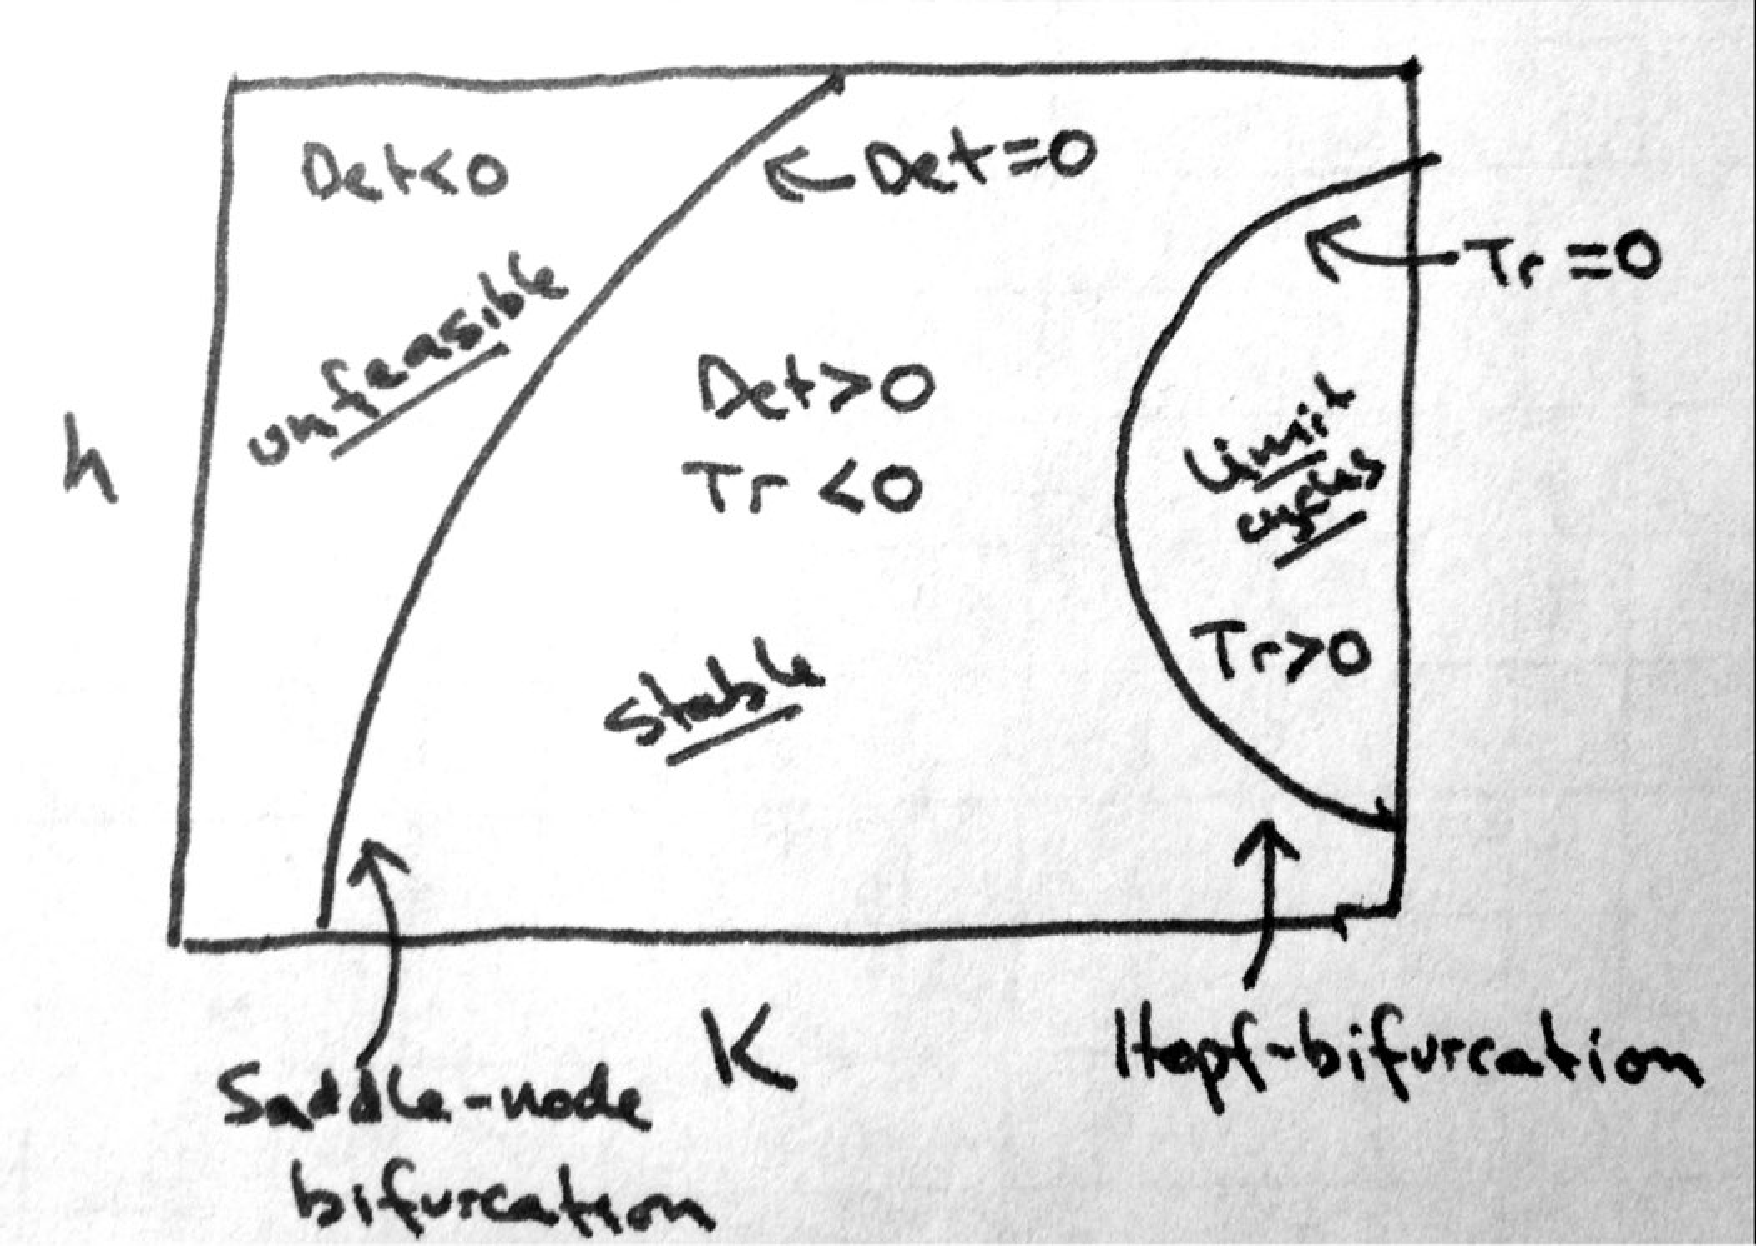
\includegraphics[width=9cm]{figs/h_v_K.pdf}\\
\end{center}

\rule[0.5ex]{\linewidth}{1pt}
\pagebreak

\textbf{Summary}: Two transitions between stability to local `instability' (two bifurcation types)
\begin{equation*}
	\lambda = \tfrac{1}{2}\text{Tr}(\textbf{A}) \pm \tfrac{1}{2}\sqrt{(-\text{Tr}(\textbf{A}))^2 - 4\cdot\text{Det}(\textbf{A})} 
\end{equation*}

\begin{minipage}[t]{\dimexpr.5\textwidth-.5\columnsep}
\textbf{Extinction of consumer:}\\
\ind $\lambda$ has only real part\\
\ind \ind $\text{Tr}(\textbf{A})^2 > 4\cdot\text{Det}(\textbf{A})$\\
\ind Transition at:\\
\ind \ind $\lambda = 0$\\
\ind \ind $ Det(\mathbf{A})=0$\\
\ind \ind $Tr(\mathbf{A}) \text{ can be } < \text{ or } > 0$\\

\textbf{Result:}\\
Qualitative change in type of steady-state.\\
Disappearance of fixed point equilibrium.\\
Appearance of new (boundary) equilibrium.\\

\ind $\Rightarrow$ \emph{Saddle-node bifurcation} $\Leftarrow$
\end{minipage} %
\begin{minipage}[t]{\dimexpr.5\textwidth-.5\columnsep}
\textbf{Emergence of limit cycle}\\
\ind $\lambda$ is complex\\
\ind \ind $\text{Tr}(\textbf{A})^2 < 4\cdot\text{Det}(\mathbf{A})$\\
\ind Transition at:\\
\ind \ind $\lambda = 0 \pm i \sqrt{\#}$\\
\ind \ind $Det(\mathbf{A})>0$\\
\ind \ind $Tr(\mathbf{A})=0$\\

\textbf{Result:}\\
Transition between damped oscillations\\
\ind to sustained oscillations.\\
Equilibrium doesn't disappear.\\

\ind \ind $\Rightarrow$ \emph{Hopf bifurcation}  $\Leftarrow$
\end{minipage}

\begin{center}
  	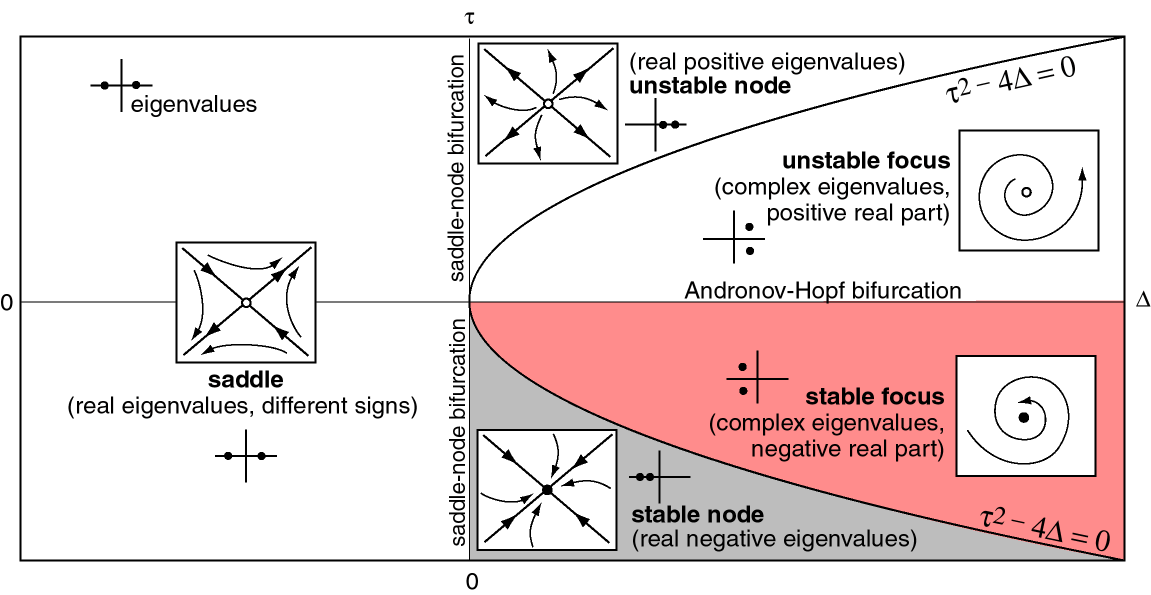
\includegraphics[width=16cm]{figs/Tr_v_Det.png}
\end{center}


\rule[0.5ex]{\linewidth}{1pt}
\rule[0.5ex]{\linewidth}{1pt}



\end{document}